%%%%%%%%%%%%%%%%%%%%% chapter.tex %%%%%%%%%%%%%%%%%%%%%%%%%%%%%%%%%
%
% sample chapter
%
% Use this file as a template for your own input.
%
%%%%%%%%%%%%%%%%%%%%%%%% Springer-Verlag %%%%%%%%%%%%%%%%%%%%%%%%%%
%\motto{Use the template \emph{chapter.tex} to style the various elements of your chapter content.}
\chapter{Linear Regression}
\label{intro} % Always give a unique label
% use \chaptermark{}
% to alter or adjust the chapter heading in the running head

\abstract*{
    This chapter introduces the principles of linear regression as a foundation for understanding the connection between differential geometry and machine learning. A simple linear model $M(x) = x\cdot W + b$ is constructed, and a loss function is used to quantify prediction errors. The chapter details the derivation of gradients for the loss with respect to the model parameters $W$ and $b$, providing insights into how these gradients guide the optimization process.
}

\abstract{
    This chapter introduces the principles of linear regression as a foundation for understanding the connection between differential geometry and machine learning. A simple linear model $M(x) = x\cdot W + b$ is constructed, and a loss function is used to quantify prediction errors. The chapter details the derivation of gradients for the loss with respect to the model parameters $W$ and $b$, providing insights into how these gradients guide the optimization process.
}

\section{Linear Models}
\label{sec:1}
Linear regressions are a fundamental tool in statistics and machine learning for modeling the relationship between a dependent variable $y$ and one or more independent variables $x$. The simplest form of linear regression is a univariate linear model\index{linear model, univariate}, which assumes a linear relationship between $y$ and $x$ of the form $y = x\cdot W + b$, where $W,b\in\mathbb{R}$ are real numbers. The model parameters $W$ and $b$ are learned from a dataset of input-output pairs $\{(x_i, y_i)\}_{i=1}^N$ by minimizing a loss function that quantifies the prediction errors of the model. 

Let's define a more general version of the linear model. 
Suppose we have $n$ samples, each with $d$ features, and our target is to predict $m$ outputs for each sample. We can represent the input data as a matrix $X\in\mathbb{R}^{n\times d}$ and the output data as a matrix $Y\in\mathbb{R}^{n\times m}$.

The linear model $M(X)$ is then defined as:
$$M(X) = X\cdot W^\T+b,$$
where:
\begin{itemize}
    \item $X\in \R^{n\times d}$ is the input matrix,
    \item $W\in\R^{m\times d}$ is the weight matrix,
    \item $b \in \R^{n\times m}$ is the bias matrix. 
\end{itemize}

The bias matrix $b$ is constructed from the bias vector $\vec{b}\in\R^{m}$ by replicating it $n$ times. In other words, each row of the bias matrix $b$ is the bias vector $\vec{b}$. $\vec{b}$ is said to be \emph{broadcasted}\index{broadcast} to the shape of $b$.


\section{Univariate Linear Models}
\label{sec:2}
Let's construct some data to work with that follows a somewhat linear trend and build a machine-learning model from scratch. We'll take the function $f(x)=x^2+2\cdot x+1$ over a random sample of points in $[0,10]$ and add some uniform noise. Next, we'll separate the synthetic data into training and test sets. This will allow us to train the model on the training data and evaluate its performance on the test data. Once we feel confident in the performance of our model, we may train using the entire dataset. For splitting, we'll use the \texttt{train\_test\_split} function from the \texttt{sklearn} library.

\lstinputlisting[language=Python]{Regression/code/1.1.1.1.py}

\begin{figure}[H]
\centering
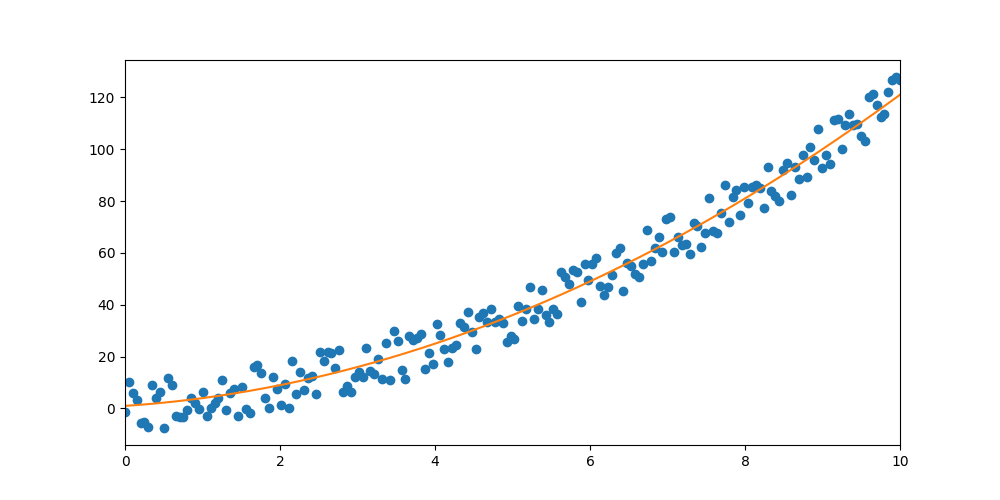
\includegraphics[width=300pt]{Regression/code/fig1.png}
\caption{Data generated from the function $f(x)=x^2+2\cdot x+1$ with added noise.}
\label{fig:linear1}
\end{figure}

In Figure \ref{fig:linear1}, the \textit{best fit} for this data is the function we used to construct it. Of course, we usually don't know the equation for the best fit beforehand, but our goal is to create a model to approximate this line as closely as possible. 

Let us start by constructing a simple machine-learning model for linear regression with no hidden layers, which essentially means there are no intermediate computations between the input and the output in our model.

Our goal is to build a machine-learning model 
$M:[0,10]\to\mathbb{R}$ of the form $$M(x) = x\cdot W + b,$$ where $W\in\mathbb{R}$ and $b\in\mathbb{R}$. Here, $W$ is called the \emph{weight} and $b$ is called the \emph{bias}.   

Here, we define our linear model:

\lstinputlisting[language=Python]{Regression/code/1.1.1.2.py}

In machine-learning, a model is initialized with random weights and biases, which are then corrected during training by minimizing a \emph{loss function}. Let's start by choosing some random $W$ and $b$.

\lstinputlisting[language=Python]{Regression/code/1.1.1.3.py}
\texttt{\small{Initial weight: 0.5136609336515561\\
Initial bias: 0.39026605372156786
}}

Given that the weight and bias was chosen at random, we don't expect it to perform very well on our data, and indeed that is the case, as shown in Figure \ref{fig:linear2}.

\begin{figure}[h]
    \centering
    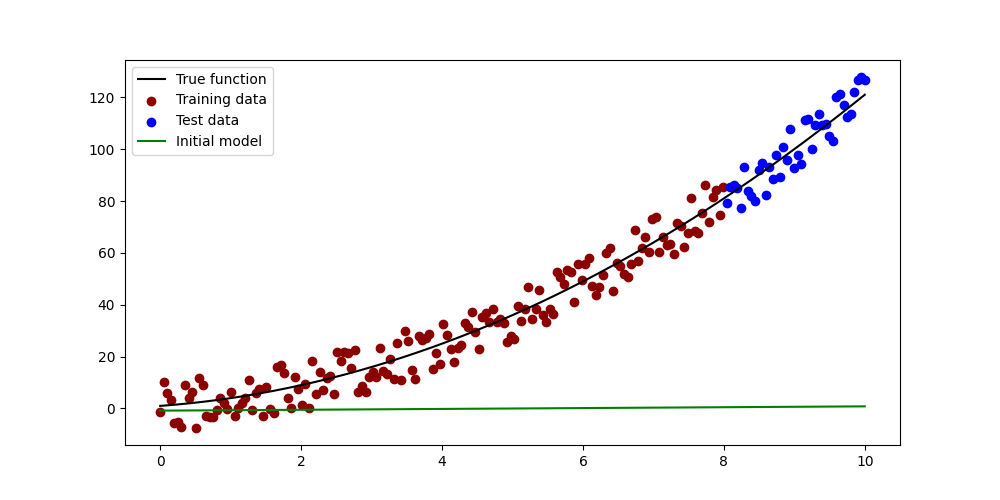
\includegraphics[width=300pt]{Regression/code/fig2.png}
    \caption{Initial model prediction with random weight and bias.}
    \label{fig:linear2}
\end{figure}

Let's work on improving the model. Improving our model will involve tweaking $W$ and $b$ to better fit the model using a process called \textbf{gradient descent}\index{gradient descent}.

\subsection{Gradient Descent for Univariate Linear Models}
\label{subsec:2}
We first define a \textbf{loss function}\index{loss function} to measure how our model is performing. This function will quantify the difference between the model's predictions and the actual data. A common loss function for linear regression is the \textit{Mean Squared Error}\index{Mean Squared Error (MSE)} (MSE), which is defined as:
\begin{equation}
\label{eq:mse}
\mathcal{L}(Y_{\text{pred}},Y) = \frac{1}{n}\|Y_\text{pred} - Y\|^2 = \frac{1}{n}\sum_{i=1}^n (y_{\text{pred}}^{(i)}-y^{(i)})^2,
\end{equation}

where:
\begin{itemize}
    \item $Y_{\text{pred}},Y \in \R^n$ are the predicted and true values, respectively, 
    \item $n$ is the number of samples,
    \item $y_{\text{pred}}^{(i)}$ and $y^{(i)}$ are the predicted and true values for the $i$-th sample, respectively.
\end{itemize}

This loss function penalizes large deviations of $Y_\text{pred}$ from $Y$ by squaring the differences.

\lstinputlisting[language=Python]{Regression/code/1.1.1.5.py}
\texttt{50th sample target: -3.2562046439706913\\
50th prediction: 0.7774476620016353\\
Loss at 50th sample: 16.270350925475867\\
Total Loss over all samples: 2899.2086153263763
} 
\linebreak

Our goal is to minimize this loss function. 

One thing to note about this loss function is that it is a differentiable function. Recal from vector calculus that the \textbf{gradient}\index{gradient} of a differentiable funtion $f$ is a vector field $\nabla f$ whose value at point $p$ is a vector that points towards the direction of steepest ascent. 

Understanding the gradients of the loss function with respect to the model parameters—specifically, the weight $W$ and bias $b$—is crucial in machine learning, particularly when employing optimization techniques like gradient descent. Our goal is to minimize the loss function. 

The gradients $\frac{\partial \mathcal{L}}{\partial W}$ and $\frac{\partial \mathcal{L}}{\partial b}$ indicate how sensitive the loss function $\mathcal{L}$ is to changes in the parameters $W$ and $b$. In essence, they provide the direction and rate at which $\mathcal{L}$ increases or decreases as we adjust these parameters.

By computing these gradients, we can iteratively update $W$ and $b$ to minimize the loss function, thereby improving the model's performance. This process is the foundation of the gradient descent optimization algorithm.


\subsubsection{Gradients}
\begin{enumerate}
    \item \textit{Gradient with Respect to Weight \( W \):}

    The partial derivative \( \frac{\partial \mathcal{L}}{\partial W} \) measures how the loss changes with respect to the weight \( W \). A positive derivative suggests that increasing \( W \) will increase the loss, while a negative derivative indicates that increasing \( W \) will decrease the loss. By moving \( W \) in the direction opposite to the gradient, we can reduce the loss.

    For the \( i \)-th data point, let \( y_\text{pred}^{(i)} = x_i \cdot W^\top + b \) be the predicted value while \( y^{(i)} \) denotes the true value. Mathematically, this gradient is computed as:
    \begin{align*}
        \frac{\partial \mathcal{L}}{\partial W} &= \frac{\partial}{\partial W} \left( \frac{1}{n} \sum_{i=1}^n (y_\text{pred}^{(i)} - y^{(i)})^2 \right) \\
        &= \frac{1}{n} \sum_{i=1}^n \frac{\partial}{\partial W} \left( (x_i \cdot W^\top + b - y^{(i)})^2 \right) \quad \text{(Substitute model equation)} \\
        &= \frac{1}{n} \sum_{i=1}^n 2 \cdot (y_\text{pred}^{(i)} - y^{(i)}) \cdot x_i \quad \text{(Chain rule)} \\
        &= \frac{2}{n} \sum_{i=1}^n (y_\text{pred}^{(i)} - y^{(i)}) \cdot x_i.
    \end{align*}

    Thus, we find that:
    \begin{equation}
    \label{eq:gradient-w}
    \frac{\partial \mathcal{L}}{\partial W} = \frac{2}{n} \sum_{i=1}^n (y_\text{pred}^{(i)} - y^{(i)}) \cdot x_i,
    \end{equation}
    or equivalently in matrix form:
    \begin{equation}
    \label{eq:gradient-w-matrix}
    \frac{\partial \mathcal{L}}{\partial W} = \frac{2}{n} \left( Y_{\text{pred}} - Y \right)^\top X,
    \end{equation}
    where \( X \) is the input matrix of shape \( n \times d \), and \( Y_{\text{pred}}, Y \in \mathbb{R}^n \).

    \item \textit{Gradient with Respect to Bias \( b \):}

    Similarly, the partial derivative \( \frac{\partial \mathcal{L}}{\partial b} \) measures how the loss changes with respect to the bias \( b \). Adjusting \( b \) in the direction opposite to this gradient will help minimize the loss.

    This gradient is computed as:
    \[
        \frac{\partial \mathcal{L}}{\partial b} = \frac{\partial}{\partial b} \left( \frac{1}{n} \sum_{i=1}^n (y_\text{pred}^{(i)} - y^{(i)})^2 \right),
    \]
    which simplifies to:
    \begin{equation}
    \label{eq:gradient-b}
    \frac{\partial \mathcal{L}}{\partial b} = \frac{2}{n} \sum_{i=1}^n (y_\text{pred}^{(i)} - y^{(i)}),
    \end{equation}
    or equivalently:
    \begin{equation}
    \label{eq:gradient-b-matrix}
    \frac{\partial \mathcal{L}}{\partial b} = \frac{2}{n} \mathbf{1}^\top \left( Y_{\text{pred}} - Y \right),
    \end{equation}
    where \( \mathbf{1} \) is a vector of ones of size \( n \).

    Proof of this equation is left as an exercise for the reader.
\end{enumerate}


With that, we can compute the gradients in Python:

\lstinputlisting[language=Python]{Regression/code/1.1.1.6.py}

Now that we have a way of computing the partial derivatives of $\mathcal{L}$ with respect to $W$ and $b$, we can visualize the \textit{gradient field}\index{gradient field}. For a given $p=(W, b) \in \mathbb{R}^2$, the gradient $\nabla \mathcal{L}$ at $p$ is a vector that points towards the rate of fastest increase. In the following code, we compute these vectors on a grid. We also include a 2D contour plot of the loss function $\mathcal{L}$. Our initial weight $W$ and bias $b$ are marked on the plot by a red dot.

\lstinputlisting[language=Python]{Regression/code/1.1.1.7.py}

\begin{figure}
    \centering
    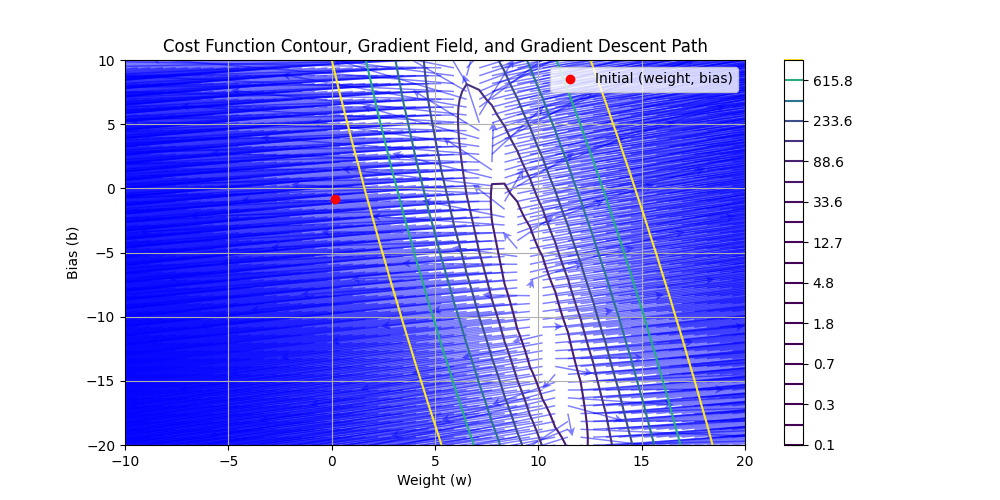
\includegraphics[width=330pt]{Regression/code/gradient-field-1.png}
    \caption{Contour plot of the loss function, gradient field, and gradient descent path.}
    \label{fig:linear3}
\end{figure}
    
Since our goal is to minimize the loss function and these vectors are pointing towards the steepest ascent of the loss function with respect to $W$ and $b$, we minimize by moving in the opposite direction of the gradients. This process is fundamental to optimization algorithms like gradient descent and is refered to as \textbf{backpropagation}\index{backpropagation} in the realm of machine-learning.

\subsubsection{Gradient Descent \& Backward Propagation}
\label{subsubsec:2}
\textbf{Gradient descent}\index{gradient descent} is an optimization algorithm that iteratively updates the model parameters in the direction opposite to the gradients of the loss function. This process continues until the loss is minimized. \textbf{Backpropagation} is the process of computing these gradients and updating the model parameters.

The parameter updates are performed iteratively using the following rules:
\begin{enumerate}
    \item  Weight update:
    $$W \leftarrow W - \alpha \frac{\partial \mathcal{L}}{\partial W}$$
   Here, $\alpha$ is the learning rate, a hyperparameter that controls the step size of each update. The term $\frac{\partial \mathcal{L}}{\partial W}$ represents the gradient of the loss function with respect to the weight. By subtracting this scaled gradient from the current weight, we move $ W $ in the direction that decreases the loss.

    \item Bias update:
    $$b \leftarrow b - \alpha \frac{\partial \mathcal{L}}{\partial b}$$
    Similarly, $\frac{\partial \mathcal{L}}{\partial b}$ is the gradient of the loss function with respect to the bias. Updating $b$ in this manner adjusts the model's predictions to better fit the data.
\end{enumerate}

The \textbf{learning rate} determines how large a step we take in the direction of the negative gradient. A small $\alpha$ leads to slow convergence, while a large $\alpha$ might cause overshooting the minimum, leading to divergence. Choosing an appropriate learning rate is crucial for effective training.

The gradients $\frac{\partial \mathcal{L}}{\partial W}$ and $\frac{\partial \mathcal{L}}{\partial b}$ indicate the direction in which the loss function increases most rapidly. By moving in the opposite direction (hence the subtraction), we aim to find the parameters that minimize the loss.

We repeat this process over and over again. Each time we do it is referred to as an \textbf{epoch}\index{epoch}. 

\lstinputlisting[language=Python]{Regression/code/1.1.1.8.py}

\texttt{\small{Initial (weight, bias): (0.5136609336515561, 0.39026605372156786)\\
Final (weight, bias): (10.472640107432522, -5.487933673141372)
}}

\begin{figure}[H]
    \centering
    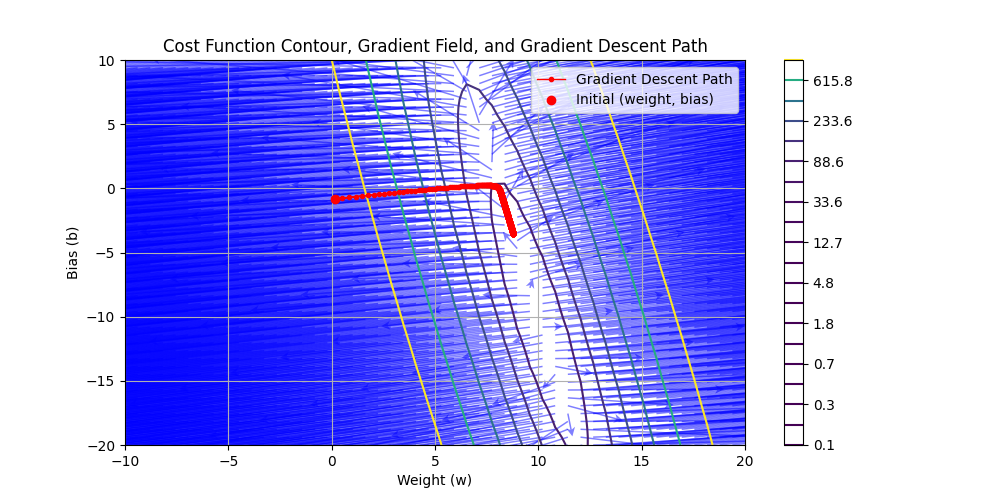
\includegraphics[width=330pt]{Regression/code/gradient-field-2.png}
    \caption{Contour plot of the loss function, gradient field, and gradient descent path.}
    \label{fig:linear4}
\end{figure}

Since our weight $W$ and bias $b$ together form a point $(W,b)\in\mathbb{R}^2$, the loss function $\mathcal{L}$ forms a 3-dimensional surface. The visualization below shows the path taken during gradient descent on the surface of the loss function $\mathcal{L}$. The initial point $(W,b)$ is in green. The path moves towards $\mathcal{L}$'s minimum. 

\begin{figure}[H]
\centering
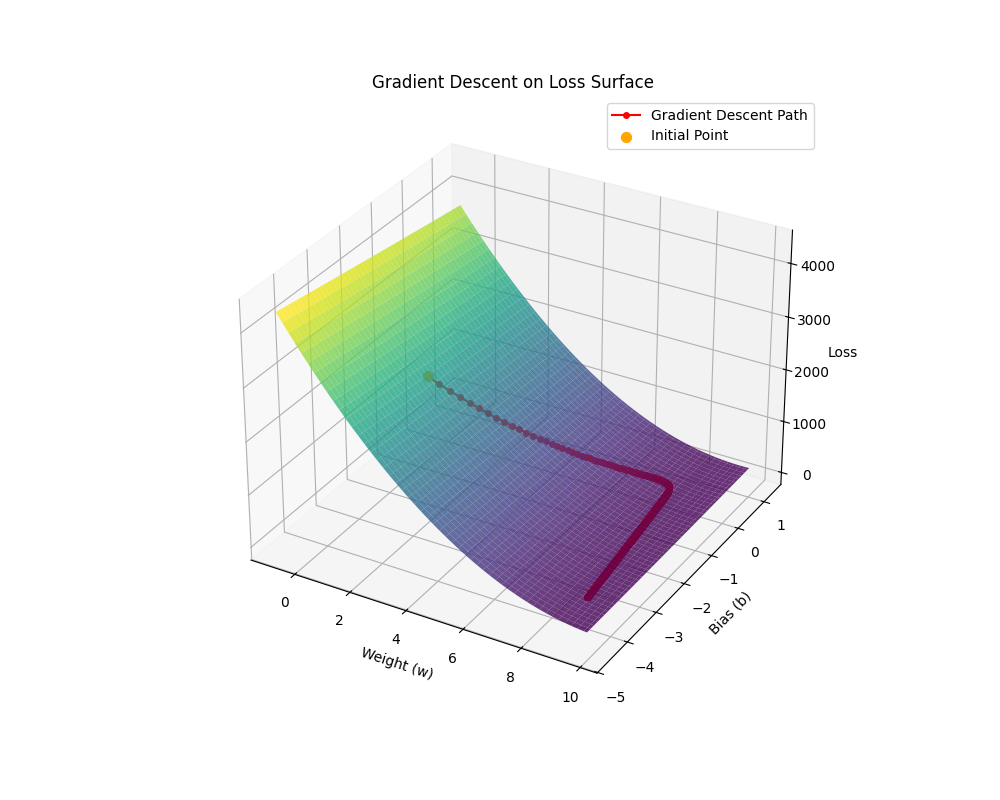
\includegraphics[width=330pt]{Regression/code/gradient-descent-3d.png}
\caption{Gradient descent path on the loss function surface. The code used to generate this visualization can be found in \ref{sec:gradient-descent-3d} of the Appendix.}
\label{fig:linear5}
\end{figure}

Finally, we visualize our initial (green) and final (red) linear model on a graph, alongside the data and true line of best fit (orange). 

\begin{figure}[H]
\centering
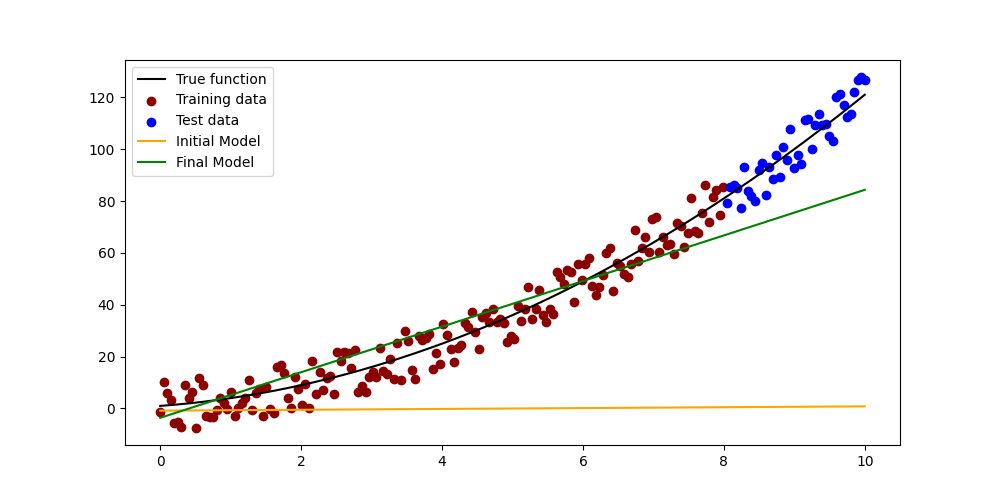
\includegraphics[width=300pt]{Regression/code/final-model.png}
\caption{Initial and final linear models compared to the true line of best fit.}
\label{fig:linear6}
\end{figure}

\subsection{Univariate Linear Models with Hidden Layers}
We build upon the ideas from the previous section by incorporating a \emph{hidden layer}\index{hidden layer} into our model, allowing it to learn intermediate representations and capture more complex patters in the data. The reason why we call it a hidden layer is because it is not directly connected to the input or output of the model. This technique involves embedding our data into higher-dimensional spaces. Higher-dimensional spaces allow for the transformation of data in a way that makes patterns, relationships, or structures more linearly separable. In lower dimensions, data that appears entangled or inseparable can often be separated in a higher-dimensional space. 

A classic example that demonstrates the concept of non-linear separability in lower dimensions but linear separability in higher dimensions is the \emph{circle classification problem}. Here, data points inside a circle belong to one class, while those outside belong to another. This problem is not linearly separable in two dimensions, but becomes linearly separable when mapped to higher-dimensional spaces using the radius as a new feature. See \ref{sec:circle-classification-visualizations} in the Appendix for the code used to generate the visualizations below.

% two figures side-by-side
\begin{figure}[H]
    \centering
    \begin{minipage}{.5\textwidth}
      \centering
      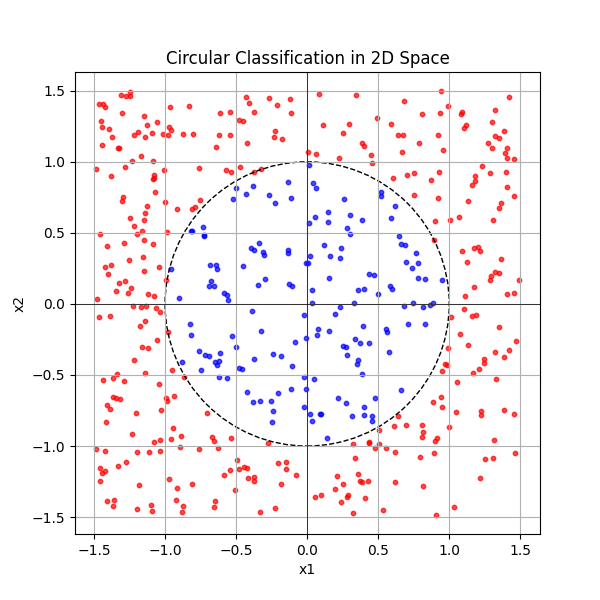
\includegraphics[width=200pt]{Regression/code/circular-data.png}
      \caption{Circle classification problem in 2D.}
      \label{fig:linear7}
    \end{minipage}%
    \begin{minipage}{.5\textwidth}
      \centering
      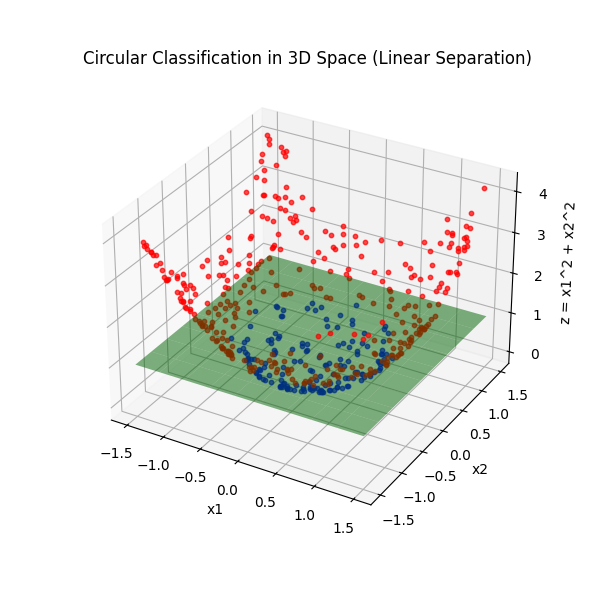
\includegraphics[width=200pt]{Regression/code/circular-data-3d.png}
      \caption{Circle classification problem in 3D.}
      \label{fig:linear8}
    \end{minipage}
\end{figure}

\subsection*{Model with a Hidden Layer}

To extend the linear model to include a hidden layer, we define the architecture mathematically as follows:

\begin{enumerate}
    \item \textbf{Input Layer:}
    \begin{itemize}
        \item The input matrix \( X \in \mathbb{R}^{n \times d} \) represents a batch of \( n \) samples, where each row corresponds to one data sample, and \( d \) is the number of input features.
        \item For inference, the model operates on a single sample (a row vector \( x \in \mathbb{R}^{1 \times d} \)) (see \ref{sec:training-with-batches} in the Appendix for why inference on a single sample works even though the model is trained on batches).
    \end{itemize}

    \item \textbf{Hidden Layer:}
    \begin{itemize}
        \item The hidden layer applies a linear transformation followed by a non-linear activation. Mathematically:
        \[
        Z_1 = X W_1 + \mathbf{1} b_1^\top,
        \]
        where:
        \begin{itemize}
            \item \( W_1 \in \mathbb{R}^{d \times h} \) is the weight matrix,
            \item \( b_1 \in \mathbb{R}^{h} \) is the bias vector (broadcasted across all samples),
            \item \( \mathbf{1} \in \mathbb{R}^{n \times 1} \) is a column vector of ones to handle the broadcast addition,
            \item \( Z_1 \in \mathbb{R}^{n \times h} \) is the resulting matrix after the linear transformation.
        \end{itemize}
        The dimension $h$ is referred to as the \emph{hidden dimension}\index{hidden dimension}, or \texttt{hidden\_dim}.
        \item A non-linear activation function \( \sigma \) is applied element-wise to \( Z_1 \) to produce:
        \[
        A_1 = \sigma(Z_1),
        \]
        where \( A_1 \in \mathbb{R}^{n \times h} \) is the activation output. We will discuss activation functions in more detail later.
    \end{itemize}

    \item \textbf{Output Layer:}
    \begin{itemize}
        \item The output layer applies another linear transformation to the hidden representation \( A_1 \), mapping it to the final prediction:
        \[
        Z_2 = A_1 W_2 + \mathbf{1} b_2,
        \]
        where:
        \begin{itemize}
            \item \( W_2 \in \mathbb{R}^{h \times m} \) is the weight matrix,
            \item \( b_2 \in \mathbb{R}^{m} \) is the bias vector (broadcasted across all samples),
            \item \( Z_2 \in \mathbb{R}^{n \times m} \) is the intermediate output before any final activation.
        \end{itemize}
        \item If a final activation function \( \phi \) is applied, the prediction becomes:
        \[
        Y_{\text{pred}} = \phi(Z_2),
        \]
        where \( \phi \) is the activation function. For regression tasks, this step is often omitted, so:
        \[
        Y_{\text{pred}} = Z_2.
        \]
    \end{itemize}
\end{enumerate}

\subsection*{Summary of Transformations}

Given \( X \in \mathbb{R}^{n \times d} \), the transformations in the model are:
\begin{enumerate}
    \item Hidden Layer:
    \[
    Z_1 = X W_1 + \mathbf{1} b_1^\top, \quad A_1 = \sigma(Z_1), \quad Z_1, A_1 \in \mathbb{R}^{n \times h}.
    \]
    \item Output Layer:
    \[
    Z_2 = A_1 W_2 + \mathbf{1} b_2, \quad Y_{\text{pred}} = \phi(Z_2), \quad Z_2, Y_{\text{pred}} \in \mathbb{R}^{n \times m}.
    \]
\end{enumerate}

You will often see graphs representing neural networks with nodes and edges, like the one below. Each node represents a \emph{neuron}, and each edge represents a \emph{connection} between neurons. The connections are weighted by the parameters \( W \) and \( b \). The activation functions are applied at each neuron, transforming the input data.

\begin{tikzpicture}[
    every node/.style={circle, draw, minimum size=1cm},
    layer/.style={rectangle, draw=none, minimum size=1cm},
    >=latex
]

% Input layer
\node[layer] (input_layer) at (0, 0) {Input Layer};
\node (I1) [below=1cm of input_layer] {$c_1$};
\node (I2) [below=1cm of I1] {$c_2$};
\node (I3) [below=1cm of I2] {$c_3$};

% Hidden layer
\node[layer] (hidden_layer) [right=2cm of input_layer] {Hidden Layer};
\node (H1) [right=3cm of I1] {};
\node (H2) [below=1cm of H1] {};
\node (H3) [below=1cm of H2] {};

% Output layer
\node[layer] (output_layer) [right=2cm of hidden_layer] {Output Layer};
\node (O1) [right=3cm of H2] {$y_{\text{pred}}$};

% Connections (Input to Hidden)
\draw[->] (I1) -- (H1);
\draw[->] (I1) -- (H2);
\draw[->] (I1) -- (H3);
\draw[->] (I2) -- (H1);
\draw[->] (I2) -- (H2);
\draw[->] (I2) -- (H3);
\draw[->] (I3) -- (H1);
\draw[->] (I3) -- (H2);
\draw[->] (I3) -- (H3);

% Connections (Hidden to Output)
\draw[->] (H1) -- (O1);
\draw[->] (H2) -- (O1);
\draw[->] (H3) -- (O1);

\end{tikzpicture}

The nodes labeled $c_1, \ldots, c_3$ correspond to the features (columns) of the input matrix $X\in \R^{n\times d}$. Mathematically, this layer simply passes the input features as is, preparing them for the hidden layer. In the hidden layer, each node aggregates contributions from all input features through a linear transformation. 

Truthfully, these graphs aren't necessary for understanding the model, and in fact I still have a rather difficult time interpreting them. However, they are useful for visualizing the model and understanding the flow of data through the network. To some people. 

Layers are connected by an \textbf{activation function}. Activation functions should satisfy the following criteria:
\begin{itemize}
    \item \emph{Non-linearity}: The function must be non-linear to allow the model to learn complex patterns.
    \item \emph{Differentiability}: The function should be differentiable on its domain to faciliate gradient-based optimization methods like backpropagation. When we dive into models over more abstract rings, we will see how this relates to the concept of \emph{derivations} over rings.
    \item \emph{Bounded output}: Having a bounded output helps in stabilizing the learning process and prevents extreme activations.
    \item \emph{Monotonicity}: A monotonic function ensures consistent gradients, aiding in stable and efficient training.
    \item \emph{Computational efficiency}: The function should be computationally efficient to evaluate and differentiate.
\end{itemize}

A good example of such a function is the \emph{sigmoid} activation function, defined as $$\sigma(z) = \frac{1}{1 + e^{-z}}.$$ This function maps any real number to the range $(0,1)$, making it useful for many regression and classification problems. The sigmoid function is differentiable, monotonic, and computationally efficient, making it a popular choice in neural networks.

\begin{figure}[H]
\centering
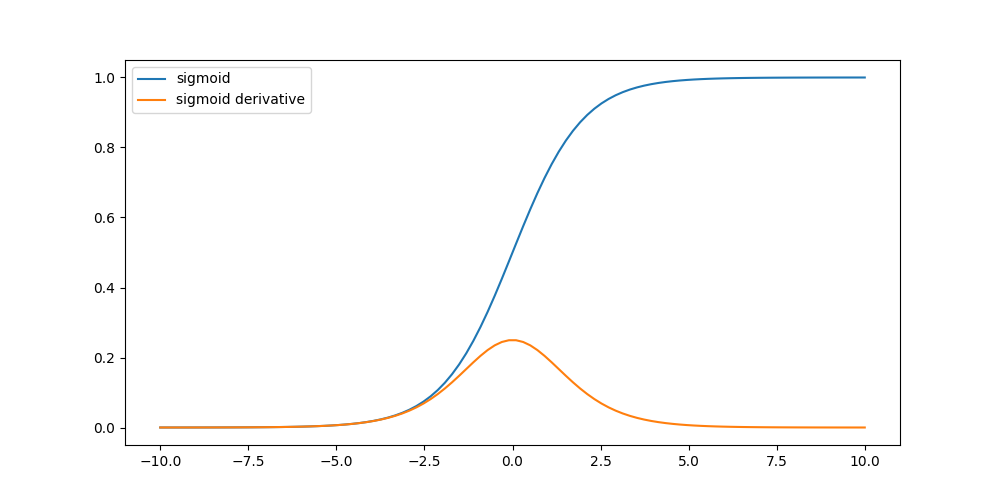
\includegraphics[width=300pt]{Regression/code/sigmoid.png}
\caption{The sigmoid activation function and its derivative.}
\label{fig:linear9}
\end{figure}

Let's implement a univariate linear model with a hidden layer with hidden dimension $d=2$ and a sigmoid activation function. We will use the same data as before.

\lstinputlisting[language=Python]{Regression/code/1.1.1.10.py}

\begin{figure}[H]
    \centering
    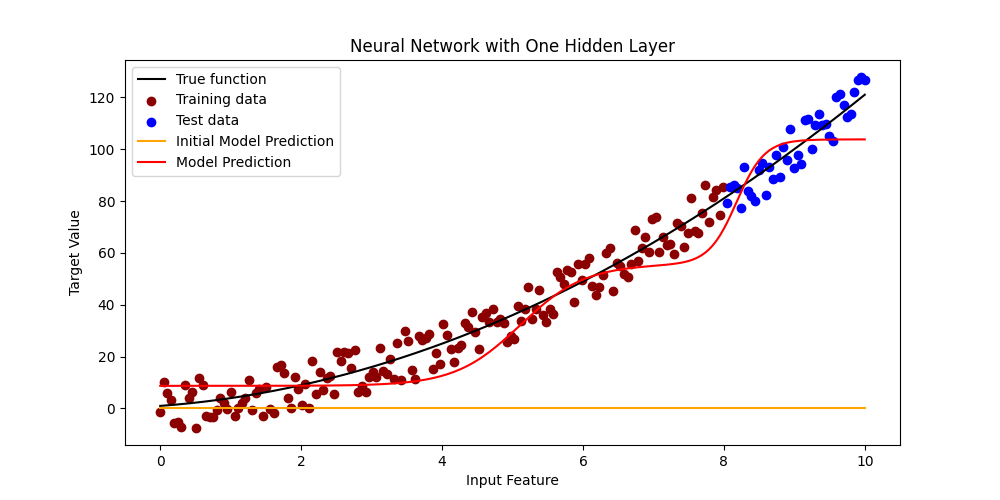
\includegraphics[width=300pt]{Regression/code/neural-network1.png}
    \caption{Univariate linear model with a single hidden layer of dimension $d=2$. The initial model's state is shown, as well as its final state after training.}
    \label{fig:linear10}
\end{figure}

As you can see, the model has learned that the data is not linear and has adjusted its weights and biases to better fit the data. 

Now let's train a similar model but with a hidden dimension of $d=10$.

\lstinputlisting[language=Python]{Regression/code/1.1.1.11.py}

\begin{figure}[H]
\centering
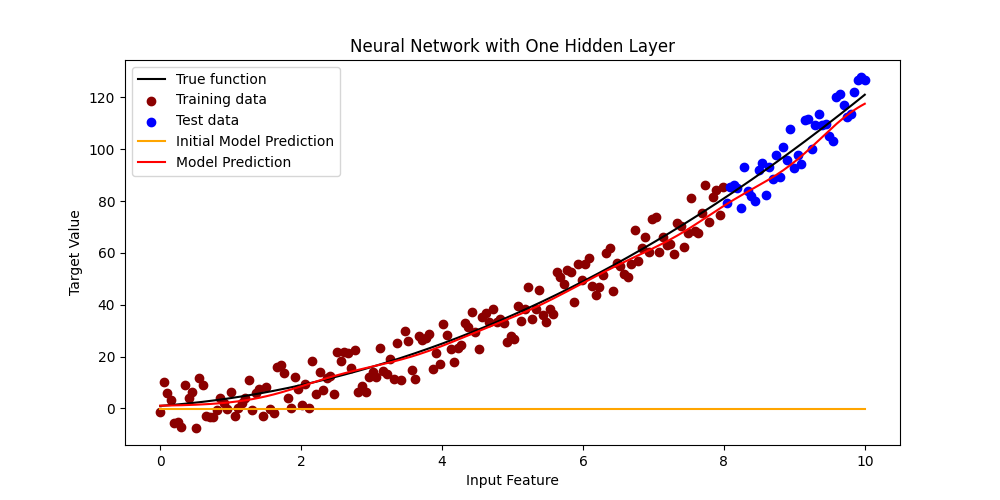
\includegraphics[width=300pt]{Regression/code/neural-network2.png}
\caption{Univariate linear model with a single hidden layer of dimension $d=10$. The initial model's state is shown, as well as its final state after training.}
\label{fig:linear11}
\end{figure}

As you can see, the higher-dimensional hidden layer allows the model to learn more complex patterns in the data and follows the true line of best fit more closely than the model with $d=2$. Furthermore, it also performs well on the test data which was excluded during training. 

\section{Multivariate Linear Models}
The next step in our journey is the multivariate linear model with no hidden layers. This model is an extension of the univariate model, allowing for multiple input features. The model definition is the same as that of the univarite case:
$$M(x) = W^\T\cdot x + b,$$
where:
\begin{itemize}
    \item $W$ is a \textbf{weight matrix} of shape $d \times m$,
    \item $x$ is a $d$-dimensional input vector,
    \item $b$ is an $m$-dimensional \textbf{bias vector}.
\end{itemize}
If we $n$ samples with $d$ features each, we can represent the input data as a matrix $X\in\mathbb{R}^{n\times d}$, where each row $X_i$ represents a sample. 

In the previous section, we utilized concepts from differential geometry to minimize the loss function and visualize the process of gradient descent. This was feasible since the model was simple and the loss function was differentiable. However, as we move to more complex models, we may not have the luxury offered by real-valued functions. 

Let's look at the \emph{Tips} dataset from the \texttt{seaborn} package as an example.

\begin{codeblock}
# %!pip install seaborn

# Import iris dataset using seaborn
import seaborn as sns
data = sns.load_dataset('tips')

data
\end{codeblock}

\begin{table}[ht]
    \centering
    \begin{tabular}{lrrllllr}
        \toprule
        & total\_bill & tip & sex & smoker & day & time & size \\
        \midrule
        242 & 17.82 & 1.75 & Male & No & Sat & Dinner & 2 \\
        73 & 25.28 & 5.00 & Female & Yes & Sat & Dinner & 2 \\
        43 & 9.68 & 1.32 & Male & No & Sun & Dinner & 2 \\
        86 & 13.03 & 2.00 & Male & No & Thur & Lunch & 2 \\
        105 & 15.36 & 1.64 & Male & Yes & Sat & Dinner & 2 \\
        \bottomrule
    \end{tabular}
    \caption{Sample data from \texttt{seaborn}'s \emph{Tips} dataset}
    \label{tab:sample_data}
\end{table}

Our goal is the predict the tip amount based on the information available. The first thing you'll notice is that this dataset contains non-numerical features. How would we include such features in our model?

\subsection{Encoding Categorical Data}
\label{subsec:3}

Since our machine-learning algorithm works with numerical data, we need to convert the categorical data in the dataset into a numerical format. Two common techniques for this are \textbf{one-hot encoding} and \textbf{label encoding}.

One might numerically encode the \texttt{day} column so that Sunday is 0, Monday is 1, and so on. In doing so, you are defining an \emph{encoding}, a numerical representation of the string. Your encoding is ordered in a sense. But when dealing with more general categorical data, we don't always have a natural ordering. Once we touch on the concept of \emph{Rings}, we will see that the days of the week form a ring under addition modulo 7, denoted $\Z/\Z_7$. For now, we will proceed not as mathematicians but as machine-learning engineers.

\begin{definition}
    An \textbf{embedding}\index{embedding} is a structure-preserving map from one mathematical object to another. $X$ is said to be embedded in $Y$ if there exists an injective function $f:X\to Y$ such that $f(x)=f(y)$ if and only if $x=y$. 
\end{definition}

\subsubsection{Label Encoding Categorical Data}

\textbf{Label Encoding}\index{label encoding} is a technique that assigns a unique integer to each category in the data. This method is simpler than one-hot encoding but may introduce an ordinal relationship between the categories that does not exist in the data. In essense, we are creating an embedding of the categorical data into $\Z$, the integers.

You can also encode the \texttt{day} column in the \emph{Tips} dataset using \texttt{scikit-learn}'s \texttt{LabelEncoder}:
\lstinputlisting[language=Python]{Regression/code/1.3.1.1.py}

\begin{table}[ht]
    \centering 
    \begin{tabular}{rrllllrr}
        \toprule
        total\_bill & tip & sex & smoker & day & time & size & day\_LabelEncoded \\
        \midrule
        17.59 & 2.64 & Male & No & Sat & Dinner & 3 & 1 \\
        38.07 & 4.00 & Male & No & Sun & Dinner & 3 & 2 \\
        22.76 & 3.00 & Male & No & Thur & Lunch & 2 & 3 \\
        13.81 & 2.00 & Male & No & Sun & Dinner & 2 & 2 \\
        23.95 & 2.55 & Male & No & Sun & Dinner & 2 & 2 \\
        \bottomrule
    \end{tabular}               
\end{table}

The result is \texttt{day\_LabelEncoded}, a new column that contains the encoded values for the \texttt{day} column. However, this encoding method introduces an ordinal relationship between the days that does not exist in the data. For example, Thursday was encoded as $3$ while Friday was encoded as $0$. Ths embedding doesn't preserve the ordered structure of the days of the week.

\subsubsection{{Ordinal Encoding Categorical Data}}

\textbf{Ordinal Encoding}\index{ordinal encoding} is similar to label encoding, but assigns an integer to each category in the data based on the order in which they appear. This method preserves the ordinal relationship between the categories but may introduce an artificial ranking that does not exist in the data.
\lstinputlisting[language=Python]{Regression/code/1.3.1.3.py}

\begin{table}[ht]
    \centering 
    \begin{tabular}{rrllllrrr}
        \toprule
        total\_bill & tip & sex & smoker & day & time & size & day\_LabelEncoded & day\_OrdinalEncoded \\
        \midrule
        15.42 & 1.57 & Male & No & Sun & Dinner & 2 & 2 & 3 \\
        48.33 & 9.00 & Male & No & Sat & Dinner & 4 & 1 & 2 \\
        7.74 & 1.44 & Male & Yes & Sat & Dinner & 2 & 1 & 2 \\
        18.64 & 1.36 & Female & No & Thur & Lunch & 3 & 3 & 0 \\
        34.65 & 3.68 & Male & Yes & Sun & Dinner & 4 & 2 & 3 \\
        \bottomrule
    \end{tabular}           
\end{table}

This does a better job at capturing the ordinal relationship between the days of the week since now Thursday comes before Friday. Still, it doesn't capture the cyclical nature of the days of the week. At the end of the week, we return to the beginning of the week, but our embedding doesn't reflect this. This is because our data inherits the structure of the ring we have embedded it in. In this case, we have embedded the days of the week in $\Z$, the integers, which is not cyclical. 
    

There is a third approach we could take: \emph{one-hot encoding}. It is a mathematically interesting approach.

\subsubsection{One-Hot Encoding Categorical Data}
\textbf{One-Hot Encoding}\index{one-hot encoding} is a technique that creates a binary column for each category in the data. Each column represents a category, and a 1 in that column indicates the presence of the category in the data. This method preserves the categorical nature of the data without introducing an ordinal relationship between the categories.

\lstinputlisting[language=Python]{Regression/code/1.3.1.2.py}

\begin{table}[ht]
    \centering 
    \begin{tabular}{rrllllrrrrr}
        \toprule
        total\_bill & tip & sex & smoker & day & time & size & day\_Thur & day\_Fri & day\_Sat & day\_Sun \\
        \midrule
        12.60 & 1.00 & Male & Yes & Sat & Dinner & 2 & 0 & 0 & 1 & 0 \\
        13.42 & 1.68 & Female & No & Thur & Lunch & 2 & 1 & 0 & 0 & 0 \\
        10.07 & 1.83 & Female & No & Thur & Lunch & 1 & 1 & 0 & 0 & 0 \\
        23.95 & 2.55 & Male & No & Sun & Dinner & 2 & 0 & 0 & 0 & 1 \\
        16.43 & 2.30 & Female & No & Thur & Lunch & 2 & 1 & 0 & 0 & 0 \\
        \bottomrule
        \end{tabular}
\end{table}    

One-hot encoding the day column resulted in four new columns, each representing a day of the week. For \texttt{day\_Fri}, a 1 indicates that the day is Friday, while 0 indicates that it is not. Thursday is represented by $(1,0,0,0)$, Friday by $(0,1,0,0)$, and so on.

This method preserves the categorical nature of the data without introducing an ordinal relationship between the categories. This still doesn't capture the cyclic nature of the days of the week, but it does a better job at separating the days of the week into distinct categories without introducing an ordinal relationship between them.

Let's train a multivariate linear model on the \emph{Tips} dataset using one-hot encoding. The process is similar to the univariate case, but we now have multiple input features. Our input data $X$ is now a matrix of shape $n\times d$, where $n$ is the number of samples and $d$ is the number of features, rather than a vector like in the univariate case. Still, the matrix algebra is the same. 

Our goal is to build a model that predicts the tip amount based on the available features. We've already encoded the \texttt{day} column. We'll have to encode the other features as well. As it turns out, the other features each have only two categories, so we can just encode them using label encoding, which will give us a binary column for each feature.

\lstinputlisting[language=Python]{Regression/code/1.3.1.4.py}

\texttt{sex encoding:\\
Male: 1 Female: 0\\ \\
smoker encoding:\\
Yes: 1 No: 0 \\ \\
time encoding:\\ 
Lunch: 1 Dinner: 0
}

\begin{table}[ht]
    \centering 
    \begin{tabular}{lrrrrrrrrrr}
        \toprule
        total\_bill & sex\_encoded & smoker\_encoded & time\_encoded & day\_Thur & day\_Fri & day\_Sat & day\_Sun & size & tip \\
        \midrule
        12.02 & 1 & 0 & 0 & 0 & 0 & 1 & 0 & 2 & 1.97 \\
        29.85 & 0 & 0 & 0 & 0 & 0 & 0 & 1 & 5 & 5.14 \\
        19.44 & 1 & 1 & 1 & 1 & 0 & 0 & 0 & 2 & 3.00 \\
        35.83 & 0 & 0 & 0 & 0 & 0 & 1 & 0 & 3 & 4.67 \\
        27.20 & 1 & 0 & 1 & 1 & 0 & 0 & 0 & 4 & 4.00 \\
        \vdots & \vdots & \vdots & \vdots & \vdots & \vdots & \vdots & \vdots & \vdots & \vdots\\
        \bottomrule
    \end{tabular}      
    \caption{Random sample of the encoded \emph{Tips} dataset}
    \label{tab:encoded_data}
\end{table}

Our input matrix $X$ is now a matrix of shape $n\times d$, where $n$ is the number of samples and $d$ is the number of features:

$$
X = \left(\begin{array}{cccccccccc}
    70 & 12.02 & 1 & 0 & 0 & 0 & 0 & 1 & 0 & 2 \\ 
    155 & 29.85 & 0 & 0 & 0 & 0 & 0 & 0 & 1 & 5  \\
    80 & 19.44 & 1 & 1 & 1 & 1 & 0 & 0 & 0 & 2  \\
    238 & 35.83 & 0 & 0 & 0 & 0 & 0 & 1 & 0 & 3  \\
    77 & 27.20 & 1 & 0 & 1 & 1 & 0 & 0 & 0 & 4  \\
    \vdots & & & \vdots & & & & & & \vdots
\end{array}\right)
$$

We need to create a model of the form 
$$M(X) = X\cdot W^\T+b,$$
where:
\begin{itemize}
    \item $X\in \R^{n\times d}$ is the input matrix,
    \item $W\in\R^{m\times d}$ is the weight matrix,
    \item $b \in \R^{n\times m}$ is the bias matrix, constructed by broadcasting the bias row vector $\vec{b}\in\R^m$ $n$ times.
\end{itemize}

In our current application, we have $d=9$ features, and since for each row we want to output a single number (the tip amount), we have $m=1$. Therefore, our weight matrix $W$ will be of shape $m\times d = 1\times 9$, and thus $W^\T$ will be of shape $d \times m = 9\times 1$. Our bias vector $\vec{b}\in \R^{m}=\R^1$ will be of shape $1\times 1$, and our bias matrix $b$ will be of shape $n\times 1$. 

As before, we initialize a random weight $W$ and bias $b$.

\begin{codeblock}
X = data[features].values
print(f'Shape of X: {X.shape}')

y = data[target].values
print(f'Shape of y: {y.shape}')

# Initialize random weight and bias for a linear model
import numpy as np
W = np.random.randn(X.shape[1])
print(f'Shape of W: {W.shape}')

b = np.random.randn(1)
print(f'Shape of b: {b.shape}')
\end{codeblock}
\texttt{
Shape of X: (244, 9)\\
Shape of y: (244,)\\
Shape of W: (9,)\\
Shape of b: (1,)
}

Now we need a loss function as before. We will use the mean squared error loss function, defined as:
$$\mathcal{L}(y_{\text{pred}},y) = \frac{1}{n}\sum_{i=1}^n (y_{\text{pred}}^{(i)}-y^{(i)})^2 = \frac{1}{n}\|Y_\text{pred} - Y\|^2,$$
where $y_{\text{pred}}^{(i)}=X\cdot W^\T + b$ is the predicted tip amount for the $i$-th sample, and $y^{(i)}$ is the actual tip amount for the $i$-th sample.

Though our model $M$ is taking in a matrix $X$ of size $n\times d$, it will still work on a single row with $d$ columns (see \ref{sec:training-with-batches} in the appendix). In this way, we can view our model as a map $M:\R^{d}\to\R^{m}$. 

\subsubsection{The Jacobian Matrix}
Suppose $f:\R^d \to\R^m$ is a function such that each of its first-order derivatives exists over $\R^d$. The \emph{Jacobian matrix}\index{Jacobian Matrix} of $f$ is a matrix of partial derivatives:
\begin{align}
\label{eq:jacobian}
J_f = \left(\begin{array}{cccc}
    \frac{\partial f_1}{\partial x_1} & \frac{\partial f_1}{\partial x_2} & \cdots & \frac{\partial f_1}{\partial x_d} \\
    \frac{\partial f_2}{\partial x_1} & \frac{\partial f_2}{\partial x_2} & \cdots & \frac{\partial f_2}{\partial x_d} \\
    \vdots & \vdots & \ddots & \vdots \\
    \frac{\partial f_m}{\partial x_1} & \frac{\partial f_m}{\partial x_2} & \cdots & \frac{\partial f_m}{\partial x_d}
\end{array}\right).
\end{align}

Given some point $p\in \R^d$, the Jacobian matrix evaluated at $p$ is denoted $J_f(p)$. The Jacobian matrix is a generalization of the gradient to multivariate functions. The gradient is a special case of the Jacobian matrix when $m=1$, where the Jacobian (a row vector) is the transpose of the gradient (a column vector).

\begin{example}
Suppose $f:\R^2\to\R^3$ is defined as 
$$f(x_1,x_2) = \left[\begin{array}{c}f_1(x_1,x_2) \\ f_2(x_1,x_2) \\ f_3(x_1,x_2)\end{array}\right] = \left[\begin{array}{c}x_1^2 + x_2 \\ \sin(x_1x_2) \\ e^{x_1-x_2}\end{array}\right].$$
Then the Jacobian matrix $J_f$ of $f$ is
\begin{align*}
    J_f &= \left(\begin{array}{cc}
        \frac{\partial f_1}{\partial x_1} & \frac{\partial f_1}{\partial x_2} \\
        \frac{\partial f_2}{\partial x_1} & \frac{\partial f_2}{\partial x_2} \\
        \frac{\partial f_3}{\partial x_1} & \frac{\partial f_3}{\partial x_2}
    \end{array}\right) \\
    &= \left(\begin{array}{cc}
        2x_1 & 1 \\
        x_2\cos(x_1x_2) & x_1\cos(x_1x_2) \\
        e^{x_1-x_2} & -e^{x_1-x_2}
    \end{array}\right).
\end{align*}

At the point $p=(1,2)\in \R^2$, the Jacobian matrix $J_f$ evaluated at $p$ is
$$
J_f(1,2) = \left(\begin{array}{cc}
    2 & 1 \\
    2\cos(2) & \cos(2) \\
    e^{-1} & -e^{-1}
\end{array}\right) \approx \left(\begin{array}{cc}2 & 1 \\ -0.832 & -0.416 \\ 0.367 & -0.367\end{array}\right)
$$
\end{example}

\begin{example}[Gradient of Mean Squared Error]
Let's consider the loss function (MSE) from our linear model:
$$\mathcal{L}(y_{\text{pred}},y) = \frac{1}{n}\sum_{i=1}^n (y_{\text{pred}}^{(i)}-y^{(i)})^2,$$
where $y_{\text{pred}}^{(i)} = X\cdot W^\T + b$ is the predicted tip amount for the $i$-th sample, and $y^{(i)}$ is the actual tip amount for the $i$-th sample. 

The Jacobian of $\loss$ with respect to the parameters $W$ and $b$ is:
$$J_\loss = \left(\begin{array}{c}
    \frac{\partial \loss}{\partial W} \\ \frac{\partial \loss}{\partial b} 
\end{array}\right)= 
\left(\begin{array}{c}
    \frac{2}{n}\sum_{i=1}^n (y_{\text{pred}}^{(i)}-y^{(i)})X_{i,:} \\
    \frac{2}{n}\sum_{i=1}^n (y_{\text{pred}}^{(i)}-y^{(i)})
\end{array}\right).$$
Notice that the partial derivatives are very similar to what we computed in the univariate case. The only difference is that we are now working with matrices and vectors instead of scalars.
\begin{proof}
We need to derive two partial derivatives: $\frac{\partial \loss}{\partial W}$ and $\frac{\partial \loss}{\partial b}$.
\begin{itemize}
\item \textbf{Partial Derivative with Respect to $W$:}
Using the chain rule:
$$\frac{\partial \loss}{\partial W} = \frac{\partial \loss}{\partial y_{\text{pred}}}\frac{\partial y_{\text{pred}}}{\partial W}.$$
Now, 
\begin{align*}
    \frac{\partial \loss}{\partial y_{\text{pred}}} &= \frac{1}{n}\sum_{i=1}^n 2(y_{\text{pred}}^{(i)}-y^{(i)}) = \frac{2}{n}\sum_{i=1}^n (y_{\text{pred}}^{(i)}-y^{(i)}), \\
    \frac{\partial y_{\text{pred}}}{\partial W} &= \frac{\partial}{\partial W}(X\cdot W^\T + b) = X.
\end{align*}
\item \textbf{Partial Derivative with Respect to $b$:}
\end{itemize}
\end{proof}
\end{example}

% \subsubsection{Encoding using Rings}
% Let's now approach encoding categorical data from a more abstract perspective. Let's begin by defining a \emph{ring}.

% \begin{definition}
%     A \textbf{ring}\index{ring} is a set $R$ equipped with two binary operations $+$ and $\cdot$ such that:
%     \begin{enumerate}
%         \item $(R,+)$ is an abelian group, i.e.
%         \begin{itemize}
%             \item $(a+b)+c = a+(b+c)$ for all $a,b,c\in R$ (associativity of addition),
%             \item $a+b = b+a$ for all $a,b\in R$ (commutativity of addition),
%             \item There exists an element $0\in R$ such that $a+0 = a$ for all $a\in R$ (additive identity),
%             \item For every $a\in R$, there exists an element $-a\in R$ such that $a+(-a) = 0$ (additive inverse).
%         \end{itemize}
%         \item $(R,\cdot)$ is a monoid, i.e.
%         \begin{itemize}
%             \item $(a\cdot b)\cdot c = a\cdot(b\cdot c)$ for all $a,b,c\in R$ (associativity of multiplication),
%             \item There exists an element $1\in R$ such that $a\cdot 1 = a$ for all $a\in R$ (multiplicative identity).
%         \end{itemize}
%         \item Multiplication distributes over addition: 
%         \begin{itemize}
%             \item $a\cdot(b+c) = a\cdot b + a\cdot c$ for all $a,b,c\in R$ (left distributivity).
%             \item $(a+b)\cdot c = a\cdot c + b\cdot c$ for all $a,b,c\in R$ (right distributivity).
%         \end{itemize}
%     \end{enumerate}
% \end{definition} 

% \begin{example}
%     The integers $\Z$ form a ring under addition and multiplication. The integers modulo $n$, denoted $\Z/n\Z$, also form a ring under addition and multiplication modulo $n$.
% \end{example}

% \begin{example}
%     The abelian group $\Z/\Z_2$, the integers modulo $2$, forms a ring under addition and multiplication modulo $2$. Two elements, $[x],[y]\in\Z/\Z_2$, are equivalent in $\Z/\Z_2$ if $x-y$ is divisible by $2$. For example, $[3]=[1]$ in $\Z/\Z_2$ since $3-1=2$ is divisible by $2$.
    
%     When context is clear, we drop the brackets around the equivalence classes and write $x$ instead of $[x]$, which leads to the infamous:
%     $$1 + 1 = 0.$$ Since $1 + 1 = 2$ over $\Z$ and $2 - 0=2$ is divisible by $2$, the equivalence classes $[2]=[0]$ are the same so that $[1]+[1]=[0]$ in $\Z/\Z_2$.
% \end{example}

% $\Z/\Z_2$ is a ring with only two elements: $0$ and $1$. Recall the one-hot encoding of the days of the week: Thursday was encoded as $(1,0,0,0)$, Friday as $(0,1,0,0)$, and so on. Each slot in the vector is either a $0$ or a $1$, depending on what is being encoded. This encoding embeds our categorical data into the direct product of rings:
% $$
% \prod_{i=1}^c \Z/\Z_2,
% $$
% where $c$ is the number of categories. 

% Some might refer to this as a direct sum, but this terminology should be avoided in the context of rings. While $\bigoplus_{i=1}^c \Z/\Z_2$ is valid in the category of abelian groups, in ring theory, the direct sum and direct product differ. Though for finite rings, the direct sum and direct product coincide.

% The \emph{direct sum} and \emph{direct product} are two closely related constructions that differ primarily in the context of infinite indexing sets. However, their behavior can diverge even for finite cases when we are careful about their definitions in different categories, such as rings or abelian groups (see \ref{sec:direct-sum-vs-direct-product} in the Appendix for more information).